% !TEX root = 0_main.tex
\chapter{Introduction}
\acrfull{sfe} allows two or more mutually suspicious parties to evaluate an arbitrary function on their private data.
The parties learn the output of the function without revealing any information about their private data.
An important special case of \acrshort{sfe} is its two-party version.
Formally in two-party \acrshort{sfe}, \textit{Alice} and \textit{Bob} wish to find the output of $f(a, b)$ where $a$ is Alice's private input, $b$ is Bob's, and $f(\cdot,\cdot)$ is an arbitrary function.
By far the most promising and efficient solution for two-party \acrshort{sfe} is \acrfull{gc} protocol proposed by Andrew C. Yao \cite{yao1986generate}.
In Yao's \acrshort{gc} protocol, the function $f(\cdot,\cdot)$ is represented as a Boolean circuit consisting of binary gates (e.g., AND, OR, XOR, etc.).
In this protocol, Alice encrypts (\textit{garbles}) the gates in the Boolean circuit, sends them to Bob, and then Bob decrypts (\textit{evaluates}) them to learn the output.
The intermediate values in the circuit along with the inputs are encrypted such that the parties' inputs remain private.
Secure evaluating of a Boolean circuit can also be generalized to multi-party \acrshort{sfe} \cite{goldreich1987play, ben2008fairplaymp}.

A host of privacy-preserving and security critical applications can directly benefit from a practical and efficient realization of \acrshort{sfe}, including but not limited to: biometrics matching, face recognition, image/data classification, electronic auctions and voting, remote diagnosis, secure search, and stable matching \cite{riazi2017toward, zhang2016robust, bringer2013privacy, evans2011efficient, barni2009secure, naor1999privacy, brickell2007privacy, jha2008towards}.

\section{Challenges}
While the \acrshort{gc} protocol was considered to be prohibitively expensive and practically infeasible a decade ago, today we are witnessing a surge of theoretical, algorithmic, and tool developments that have significantly improved the efficiency and practicality of this protocol, see \cite{malkhi2004fairplay, kolesnikov2008improved, pinkas2009secure, huang2011faster, bellare2013efficient, zahur2015two, zahur2015obliv, liu2015oblivm}.
However, three main challenges have yet to be addressed for a wide adoption of the \acrshort{gc} protocol in the digital world: efficiency, scalability, and ease-of-use.

\subsection{Efficiency}
Although the \acrshort{gc} protocol has a constant complexity for communication rounds that makes it superior to other \acrshort{sfe} protocols, \acrshort{gc} is still considered a communication-intensive protocol.
That means the cost of transferring encrypted data between the parties far exceeds the cost of \acrshort{gc}'s encryption/decryption (computation)  \cite{gueron2015fast}.
In \acrshort{gc}, the communication is mainly originated from transferring encrypted (garbled) gates of the Boolean circuit from Alice to Bob.
To improve the efficiency of a function's secure computation, this communication has to be decreased.
This can be achieved through reducing either the communication cost of a gate, or total number of gates in the function's Boolean circuit.

The research on the efficiency of the \acrshort{gc} protocol can be roughly classified into two categories:
(i) Optimizations of cryptographic constructs and protocols such as \cite{kolesnikov2008improved,pinkas2009secure,bellare2012foundations,bellare2013efficient,kolesnikov2014flexor,zahur2015two}; out of which, the two most prominent are Free XOR \cite{kolesnikov2008improved} and Half Gate \cite{zahur2015two}.
Free XOR shows that XOR gates in the circuit do not need to be communicated.
And the Half Gate technique reduces the communication cost of non-free (non-XOR) gates to the minimum possible cost using symmetric encryption. (Further communication reduction may only be achieved using more costly asymmetric encryptions.)
(ii) Engineering techniques including but not limited to \cite{henecka2010tasty,huang2011faster,henecka2013faster,kreuter2013pcf,franz2014cbmc,mood2016frigate}.
The main objective of these techniques was to create a framework that, given a function, generates an \textit{optimized} Boolean circuit that has minimum number of non-free gates.
They either employ library-based or compiler-based approaches.

The library-based approaches are based on building a library for a general purpose programming language such as Java along with routines for emitting the optimized sub-circuits, e.g., \cite{huang2011faster,malka2011vmcrypt,henecka2013faster}.
For better usability, their libraries typically include the manually optimized sub-circuits of frequently used operations such as adder and multiplier.
One of the drawbacks of the library-based approaches is that they do not perform optimization global circuit.

The compiler-based approaches provide users with a new domain-specific programming language to describe the function.
Along with the language, a new custom compiler is introduced to translate the described function into a Boolean circuit, e.g., \cite{malkhi2004fairplay,kreuter2012billion,kreuter2013pcf,franz2014cbmc}.

\subsection{Scalability}

For executing the \acrshort{gc} protocol, the parties have to store the encrypted input and intermediate values in their memory.
The size of this data increases linearly with the number of gates in the Boolean circuit.
Both library-based and compiler-based approaches suffer from complicated memory-management when the number of gates is large, thereby affecting their performance and scalability \cite{henecka2013faster, kreuter2013pcf}.
A number of frameworks have been recently proposed to address the scalability problem of previous methods such as \cite{malka2011vmcrypt, mood2012memory, kreuter2012billion, kreuter2013pcf}.
Unfortunately, they do not provide a generic solution that addresses both efficiency and scalability at once.

\subsection{Ease-of-use}
As mentioned earlier, \acrshort{gc} requires the function to be represented as a Boolean circuit.
Usually, users find it cumbersome to describe a fairly simple function by connecting Boolean gates to make the circuit.
To facilitate the circuit generation, the library-based frameworks provide libraries of optimized sub-circuits, so users can manually connect them together to make the circuit.
However, for creating an optimized circuit, users need to have through knowledge about digital design and the low-level structure of the circuit.

To further simplify developing application for \acrshort{sfe}, a number of compiler-based frameworks provide user with high-level languages to develop the function \cite{mood2012memory,kreuter2012billion,kreuter2013pcf,liu2015oblivm}.
Recently, a few frameworks support standard high-level languages like \gls{c} as well \cite{holzer2012secure, franz2014cbmc, zahur2015obliv, mood2016frigate}, however they do not exhibit the efficiency comparable to competitor approaches.

Despite numerous efforts in improving efficiency, scalability, and simplicity of the \acrshort{gc} protocol, none of the existing approaches addressed these three challenges at once.

\section{Our Approach}
We proposed a holistic solution to enhance the efficiency, scalability, and simplicity of the \acrshort{gc} protocol in this thesis.
Our approach has three main pillars to address these major challenges: \acrlong{gc} synthesis, sequential \acrlong{gc} and garbled processor.

\subsection{Garbled Circuit Synthesis}
Our \acrfull{gc} synthesis solution simply views the optimized circuit generation for \acrshort{gc} as an atypical logic synthesis task that, if properly defined, can still be addressed by conventional hardware synthesis tools.
By posing the circuit generation for Yao's protocol as a hardware synthesis problem, we naturally benefits from the elegant algorithms and powerful techniques already incorporated in existing logic synthesis solutions, see, \cite{sentovich1992sis,micheli1994synthesis,devadas1994logic,brayton1987mis}.
This view provides a radically different perspective on this important problem in contrast to the earlier work in this area that attempted to generate circuits by building new libraries for general purpose languages such as Java \cite{huang2011faster,malka2011vmcrypt}, custom compilers such as \cite{kreuter2013pcf,franz2014cbmc}, or introduction of new programming languages such as \cite{malkhi2004fairplay,rastogi2014wysteria}.

We introduce new techniques for minimizing the number of non-XOR gates which directly results in reducing communication cost for the \acrshort{gc} protocol.
We do so by integrating the cost function in the new custom libraries that we design and use within our logic synthesis flow.
This way, we are able to gain up to $80\%$ improvement in the number of non-XOR gates for benchmark circuits compared to \gls{pcf} \cite{kreuter2013pcf}.
Our methodology is automated, i.e., the savings can be achieved for many functions synthesized by our method, regardless of their sophistication.

Our logic synthesis method can also be applied to other circuit-based \acrshort{sfe} protocols with different cost functions, e.g., \acrfull{gmw}~\cite{goldreich1987play}, and \acrfull{bmr}~\cite{beaver1990round}.
For example, Demmler et al, showed how our \acrshort{gc} synthesis approach can be adopted and applied for the \acrshort{gmw} protocol where the cost depends on both the depth and size of the circuit~\cite{demmler2015automated}.
In this thesis, we will focus only on the \acrshort{gc} protocol and we leave the adaptation of our approaches for other circuit-based protocols to the future work.

\subsection{Sequential Garbled Circuit}
To address the scalability, we introduce sequential \acrfull{gc} which differentiates our methodology from the previous work.
Sequential \acrshort{gc} allows expressing the function in a very compact format, namely as a sequential logic.
The earlier work in this area mainly described functions in a combinational format, where the value of the output is determined entirely by the circuit inputs.
This input/output relationship can be expressed by a (combinational) Boolean function and a \acrfull{dag} of binary gates.
The sequential circuit description, on the other hand, allows having feedback from the output to the input by adding the notion of a state (memory).
At each \emph{sequential cycle}, the output of the circuit is determined by the current state of the circuit and the input.
For each particular sequential cycle, the relationship between the output and the inputs for the given states can be determined as a Boolean combinational logic.

The only previous work, we are aware of, which implicitly hinted at the possibility of having a more compact representation is \gls{pcf} \cite{kreuter2013pcf}.
It does so by embracing loops and unrolling them only at runtime.
A sequential circuit, however, goes far beyond the loop embracing performed at the software level.
Not only does our approach embrace the high-level loops, it also enables the user to further compact the functions by folding the implementation up to its basic elements.
For example, using our method, user can compress the 1024-bit addition function into only a 1-bit adder.

An important advantage of our sequential representation is providing a new degree of freedom to the user to fold the functions to simpler computing elements; i.e., the user has the freedom to choose the number of sequential cycles needed for evaluation of the function--the size of the combinational logic path between the states/inputs and the outputs.
The number of gates in the sequential circuit can be managed by varying the number of cycles.
The memory footprint of the \acrshort{gc} operation is directly related to the number of gates in the sequential circuit; at any moment during garbling/evaluation, only the information corresponding to the current cycle needs to be stored.
Compact sequential circuits yield a small enough memory footprint that can fit mostly on a typical processor cache.
This helps us to avoid costly cache misses while accessing the wire labels during the \acrshort{gc} protocol.
Indeed, our sequential \acrshort{gc} can enable practicable embedded implementations with a small memory footprint.
In \appx{chap:knn}, we implement a scalable solution for private nearest neighbor search as an application of the sequential \acrshort{gc}.

\subsection{Garbled Processor}
\subsection{Garbled Processor for PF-SFE}
The sequential representation enables, for the first time, implementation of a universal processor for private function evaluation where the function is known only to one party.
We reduce \acrfull{pf-sfe} to general \acrshort{sfe} by secure evaluation of a general-purpose processor like \gls{mips}.
\acrshort{pf-sfe} is useful for scenarios where the function is proprietary or classified, e.g., credit checking or private database queries.
Formally, the processor ($f(\cdot,\cdot)$) accepts a binary code of Alice' private function ($g_{Alice}(\cdot)$) along with Bob's private input ($b_{Bob}$).
The processor then computes the private function given the private input: $o = f(b_{Bob}, g_{Alice}(\cdot)) = g_{Alice}(b_{Bob})$.
The private function $g_{Alice}(\cdot)$ can be written in a high-level language and compiled using standard compiler into the binary code.
Since a processor is inherently a sequential circuit, the garbled processor was infeasible to be realized with previous \acrshort{gc} frameworks.

\subsection{Garbled Processor for SFE}
The garbled processor approach, beside providing a scalable solution for \acrshort{pf-sfe}, also makes developing \acrshort{sfe} applications easier and more accessible to non-expert users.
Using a garbled processor, the function is not required to be represented as Boolean circuit anymore; users are allowed to describe the function in high-level language and compile it into binary code using standard compiler.
This development flow is more similar to the conventional software development flow compared to that of previous library- and compiler-based approaches.

Unfortunately, the cost of using garbled processor for \acrshort{sfe} where the function is not private is staggeringly larger than the cost incurred by the conventional \acrshort{sfe} approaches.
This is because garbled processor always hides the function by garbling/evaluating the entire processor.
Thus, using garbled processor results in an unnecessary overhead for numerous applications in which a private function is not required.
To reduce this overhead, we extend the garbled \gls{mips} processor for \acrshort{sfe} by relaxing the privacy of the function.
We further improve garbled processor approach by proposing \gls{arm2gc} a framework based on the \gls{arm} processor that closes the gap between the cost of conventional \acrshort{sfe} approaches (e.g., \acrshort{gc} synthesis) and that of garbled processors.

\subsubsection{MIPS for SFE}
We extend garbled \gls{mips} to provide a generalized support for \acrshort{sfe} of varying flavors of privacy, beyond \acrshort{pf-sfe}, to allow for more relaxed privacy demands and hence an improved performance.
More explicitly, the parties can evaluate a private, semi-private or public function by revealing none, partial or all information about the function respectively while still benefiting from the simplicity of programming a processor.
We provide a coarse-grain optimization in which both parties decide first which subset of \gls{mips} \acrfull{isa} they are willing to use which determines the level of privacy.
The looser privacy of the function results in less number of non-XOR gates in the circuit of \gls{mips} processor.
The function $g(\cdot,\cdot)$ is described in a high-level language, e.g., \gls{c} and compiled into a binary code of \acrshort{mips}.
Next, the \gls{mips} processor $f(\cdot, \cdot, \cdot)$ is garbled/evaluated given the parties' private inputs $a$ and $b$ and the compiled binary code of $g(\cdot,\cdot)$ to compute the output $o = f(a, b, g(\cdot,\cdot)) = g(a,b)$.

\subsubsection{ARM for SFE}
We also introduce a methodology to perform fine-grain (gate-level) optimization on garbled processor such that only the gates associated to the private inputs incur garbling cost.
Our key observation is that the gates whose outputs are independent of the private data (and thus known to both parties) can either be computed without communication or simply skipped.
This observation gives birth to the novel \gls{skipgate} algorithm.
The algorithm wraps around the \acrshort{gc} protocol to compute the gate outputs that can be computed without communication and to mark the redundant gates for skipping\footnote{\gls{skipgate} avoids garbling redundant gates and is orthogonal to cryptographic methods such as Free XOR~\cite{kolesnikov2008improved} and Half Gate~\cite{zahur2015two} that reduce the garbling cost of a gate.}.

\gls{skipgate} is mostly effective for reducing the garbling cost of sequential circuits containing known control paths.
An example of such a circuit is the garbled processor where the control path depends on the binary code of the function that is known to both parties.
By utilizing this property, we develop a high-level \acrshort{gc} framework called \gls{arm2gc} built upon the \gls{arm} \acrshort{isa} and the \gls{skipgate} algorithm.
Users can develop the secure function in high-level languages, e.g., \gls{c} and compile it using standard \gls{arm} cross-compilers.
In contrast to the earlier high-level compiler-based approaches which called for new ad-hoc verification techniques~\cite{rastogi2014wysteria,demmler2015aby,liu2015oblivm,mood2016frigate}, \gls{arm2gc} inherits the \gls{arm}'s available fully verified compilers.
Thanks to \gls{skipgate}, \gls{arm2gc} incurs a garbling cost comparable to the \acrshort{gc} synthesis approach while allowing users to develop \acrshort{sfe} applications in a high-level language.

\gls{arm2gc} leverages \gls{arm} as the general purpose processor, instead of \gls{mips} because of \gls{arm}'s pervasiveness and, most importantly, conditional execution.
The latter simplifies the framework by reducing conditional branches and making the program flow predictable for both parties to take the full advantage of the \gls{skipgate} algorithm.

\section{Global Flow}
\subsection{TinyGarble}
We combined our \acrshort{gc} synthesis and sequential \acrshort{gc} approaches into a framework called \gls{tinygarble}.
\gls{tinygarble} accepts inputs in two different formats: a standard \acrfull{hdl}, or a higher-level language as long as it is compatible with the existing \acrfull{hls} tools, e.g., \gls{c} for  SPARK \cite{Gupta2004} and Xilinx Vivado \cite{tool:Vivado}, or Python for PandA \cite{tool:PandA}, that converts the high level language to an \acrshort{hdl}.
Beside user's manual optimization, \gls{tinygarble} performs various optimizations through standard logic synthesis tools to generate an optimized \emph{netlist}, i.e., list of gates, which is then transformed to \acrfull{sscd} format to be used in our implementation of the \acrshort{gc} protocol.

The global flow of \gls{tinygarble} framework is shown in \fig{fig:tinygarbel-global-flow}.
The framework consists of two main part (i) \acrshort{gc} synthesis flow and (ii) \acrshort{gc} engine.
The \acrshort{gc} synthesis flow receives a sequential description of the function ($f(\cdot, \cdot)$) in \acrshort{hdl} and generates a Boolean circuit that can be efficiently evaluated by the \acrshort{gc} protocol.
The \acrshort{gc} synthesis can generate combinational circuits as well as sequential ones.

The \acrshort{gc} engine is an implementation of the \acrshort{gc} protocol allows two parties, Alice and Bob, to securely evaluate the function $f(\cdot,\cdot)$ given the function description generated by the \acrshort{gc} synthesis flow and parties private inputs ($a$ and $b$).
By the end of the protocol, both parties learn the output $o = f(a, b)$ without learning anything about the other parties' input.
The \acrshort{gc} engine supports garbling/evaluating of sequential circuits along with the most recent \acrshort{gc}'s cryptographic optimizations~\cite{kolesnikov2008improved, bellare2013efficient, zahur2015two}.
We discuss \gls{tinygarble} \acrshort{gc} engine in more details in \appx{chap:engine}.

\begin{figure}
\centering
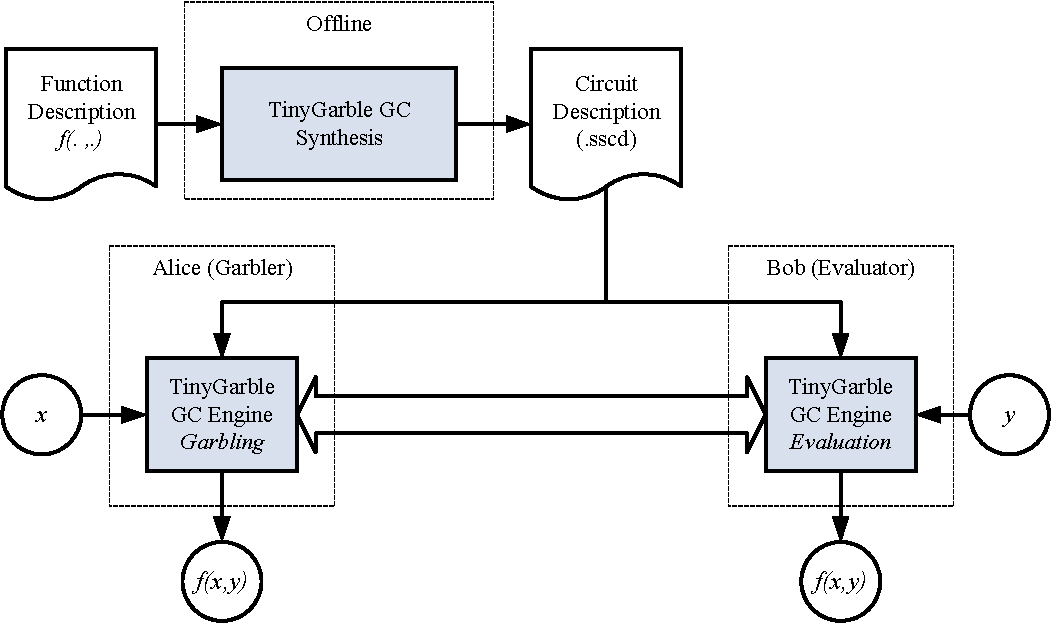
\includegraphics[width=\textwidth]{tinygarble_flow-crop.pdf}
\caption{The global flow of \gls{tinygarble} framework.
The framework consists of \acrshort{gc} synthesis flow and \acrshort{gc} engine.
The \acrshort{gc} synthesis flow generates the optimized Boolean circuit given a function description.
The \acrshort{gc} engine allows two parties (Alice and Bob) to securely compute the function according to Yao's \acrshort{gc} protocol.
}
\label{fig:tinygarbel-global-flow}
\end{figure}

\subsection{ARM2GC}
The \gls{arm2gc} framework is built upon the \gls{tinygarble} framework.
The circuit of \gls{arm} processor $f(\cdot,\cdot,\cdot)$ is synthesized using the \gls{tinygarble} \acrshort{gc} synthesis flow.
The function $g(\cdot,\cdot)$ is described by user in a high-level language ( e.g., \gls{c}) and compiled using an \gls{arm} cross-compiler (e.g., gcc-arm) to produce the binary code.
Then, the \gls{tinygarble} \acrshort{gc} engine that supports skipgate is used to securely evaluate the circuit of the \gls{arm} processor given the publicly known binary code of the function ($p=g(\cdot,\cdot)$), and parties inputs ($a$ and $b$).
By the end of the protocol, both parties revives the output of $o = f(a,b,p) = g(a,b)$ without learning anything about the other parties' input.

\begin{figure}
\centering
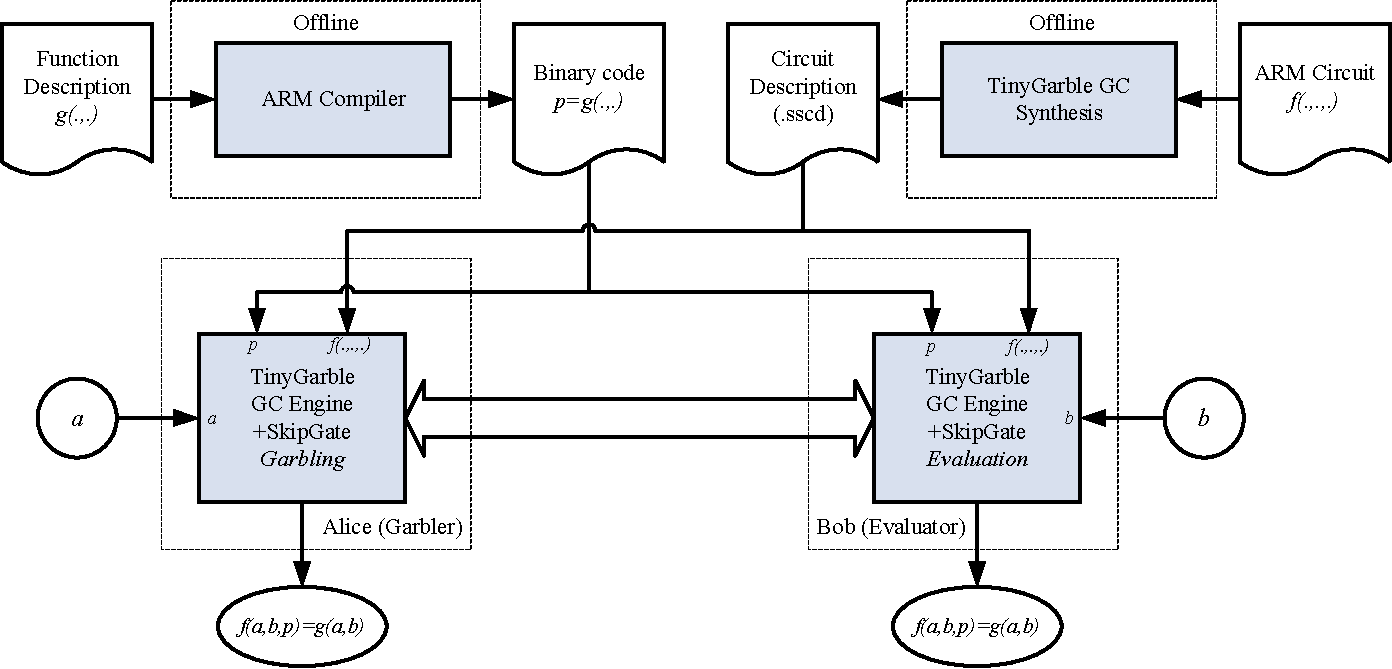
\includegraphics[width=\textwidth]{arm2gc_flow-crop.pdf}
\caption{The global flow of \gls{arm2gc} framework.
The framework consists of \acrshort{gc} synthesis flow of \gls{tinygarble} and its \acrshort{gc} engine with \gls{skipgate} algorithm.
The \acrshort{gc} synthesis flow generates the circuit description of the \gls{arm} processor $f(\cdot,\cdot,\cdot)$.
The function to be securely evaluated ($g(\cdot,\cdot)$) is compiled using an \gls{arm} cross-compiler.
The \acrshort{gc} engine allows two parties (Alice and Bob) to securely compute the \gls{arm} circuit $f(a,b,p)$ where $p$ is the binary code of $g(\cdot,\cdot)$.
At the end, they will receive the output of $f(a,b,p) = g(a,b)$
}
\label{fig:arm2gc-globalflow}
\end{figure}

\section{Contributions}
In brief, the main contributions of this thesis are as follows:
\begin{itemize}
  \item
  We address the efficiency challenge of the gc protocol by introducing \acrshort{gc} synthesis that adapts the established logic synthesis techniques to compile a function into an optimize Boolean circuit.

  \item
  We address the scalability challenge of the \acrshort{gc} protocol by introducing sequential \acrshort{gc} that allows us to achieve an unprecedented compactness in function representation and memory footprint at the same time benefiting from \acrshort{gc} synthesis optimization.

  \item
  We implement the first scalable emulation of a universal processor for private function evaluation (\acrshort{pf-sfe}) where the number of instruction invocations is not limited by the memory required for garbling.
  This design is uniquely enabled by the sequential \acrshort{gc}.
  Our design is a secure general-purpose processor based on \gls{mips} that receives the private function from one party and the data from the other.

  \item
  We propose a \gls{mips}-based garbled processor solution for \acrshort{sfe} that allows leveraging the trade-off between privacy and performance: application-specific \acrshort{isa} for \acrshort{sfe}, restricted \acrshort{isa} for semi-private \acrshort{sfe}, and full \acrshort{isa} for \acrshort{pf-sfe}.

  \item We introduce the novel \gls{skipgate} algorithm that avoids redundant garbling by utilizing the mutual knowledge between the two parties.

  \item
  We develop the \gls{arm2gc} framework based on the \gls{skipgate} algorithm and \gls{arm} processor.
  In this framework, users can efficiently develop \acrshort{sfe} applications in a high-level language like \gls{c}.
  It enables them to benefit from the available fully verified compilers of \gls{arm}.
\end{itemize}

\section{Organization}
The thesis is organized as follows.
We review the preliminaries and background of the \acrshort{sfe}, \acrshort{gc}, and Boolean circuits in \chap{chap:prelim}.
We discuss \acrshort{gc} synthesis and its limitation in \chap{chap:syn}.
Sequential \acrshort{gc} and its overhead is described in \chap{chap:seq}.
We introduce \gls{skipgate} algorithm to remove the sequential overhead in \chap{chap:skipgate}.
Next, we present garbled processors for \acrshort{pf-sfe}, \acrshort{sfe} and \gls{arm2gc} framework in \chap{chap:processor}.
Lastly, we review the related work in \chap{chap:related} and conclude the thesis in \chap{chap:conclusion}.
